\section{Pendahuluan}
\label{sec:intro}

Pasar \textit{futures} Bitcoin merupakan salah satu instrumen keuangan dengan karakteristik paling menantang untuk dimodelkan secara algoritmik. Volatilitas hariannya yang dapat mencapai 10--20\% dalam satu sesi, distribusi \textit{return} yang bercirikan \textit{fat-tail} (jauh dari asumsi Gaussian), serta sifat \textit{non-stationary} yang menyebabkan perubahan regime pasar secara mendadak --- semuanya menjadikan pendekatan \textit{machine learning} konvensional sering kali tidak memadai.

Penelitian ini mempresentasikan \textbf{BTC-QUANT}, sebuah sistem \textit{scalping} algoritmik yang dibangun di atas fondasi \textbf{ekonofisika} --- cabang ilmu yang meminjam kerangka berpikir fisika statistik untuk memodelkan dinamika pasar finansial. Kontribusi utama ekonofisika dalam sistem ini terletak pada \textbf{Layer 1: \textit{Bayesian Changepoint Detection} (BCD)}, yang memperlakukan perubahan regime pasar sebagai \textit{phase transition} --- analog dengan perubahan fase dalam sistem fisik --- alih-alih sebagai transisi probabilistik statis seperti pada model Markovian.

\subsection{Motivasi dan Rumusan Masalah}

Pertanyaan penelitian yang mendasari pengembangan BTC-QUANT adalah:
\begin{enumerate}
    \item Dapatkah pendekatan berbasis \textit{structural break} (BCD) mengungguli model \textit{clustering} global (HMM) dalam mendeteksi regime pasar kripto secara prediktif?
    \item Apakah arsitektur multi-lapis yang memisahkan deteksi regime, konfirmasi teknikal, kecerdasan buatan, dan filter volatilitas dapat menghasilkan profil risiko-pengembalian yang superior dibandingkan pendekatan \textit{single-model}?
    \item Pada titik kompleksitas mana penambahan fitur justru memperburuk performa (\textit{alpha decay})?
\end{enumerate}

\subsection{Latar Belakang: Era Hidden Markov Model}
Pada tahap awal riset, kami mencoba menerapkan \textit{Gaussian Hidden Markov Model} (HMM) untuk mendeteksi rezim pasar sesuai dengan metodologi standar dalam pengolahan sinyal \cite{rabiner1989tutorial}. Hipotesis awalnya adalah harga bersifat Markovian, di mana status pasar (bullish, bearish, sideways) dapat diestimasi dari observasi \textit{return} dan volume.

\begin{figure}[h!]
    \centering
    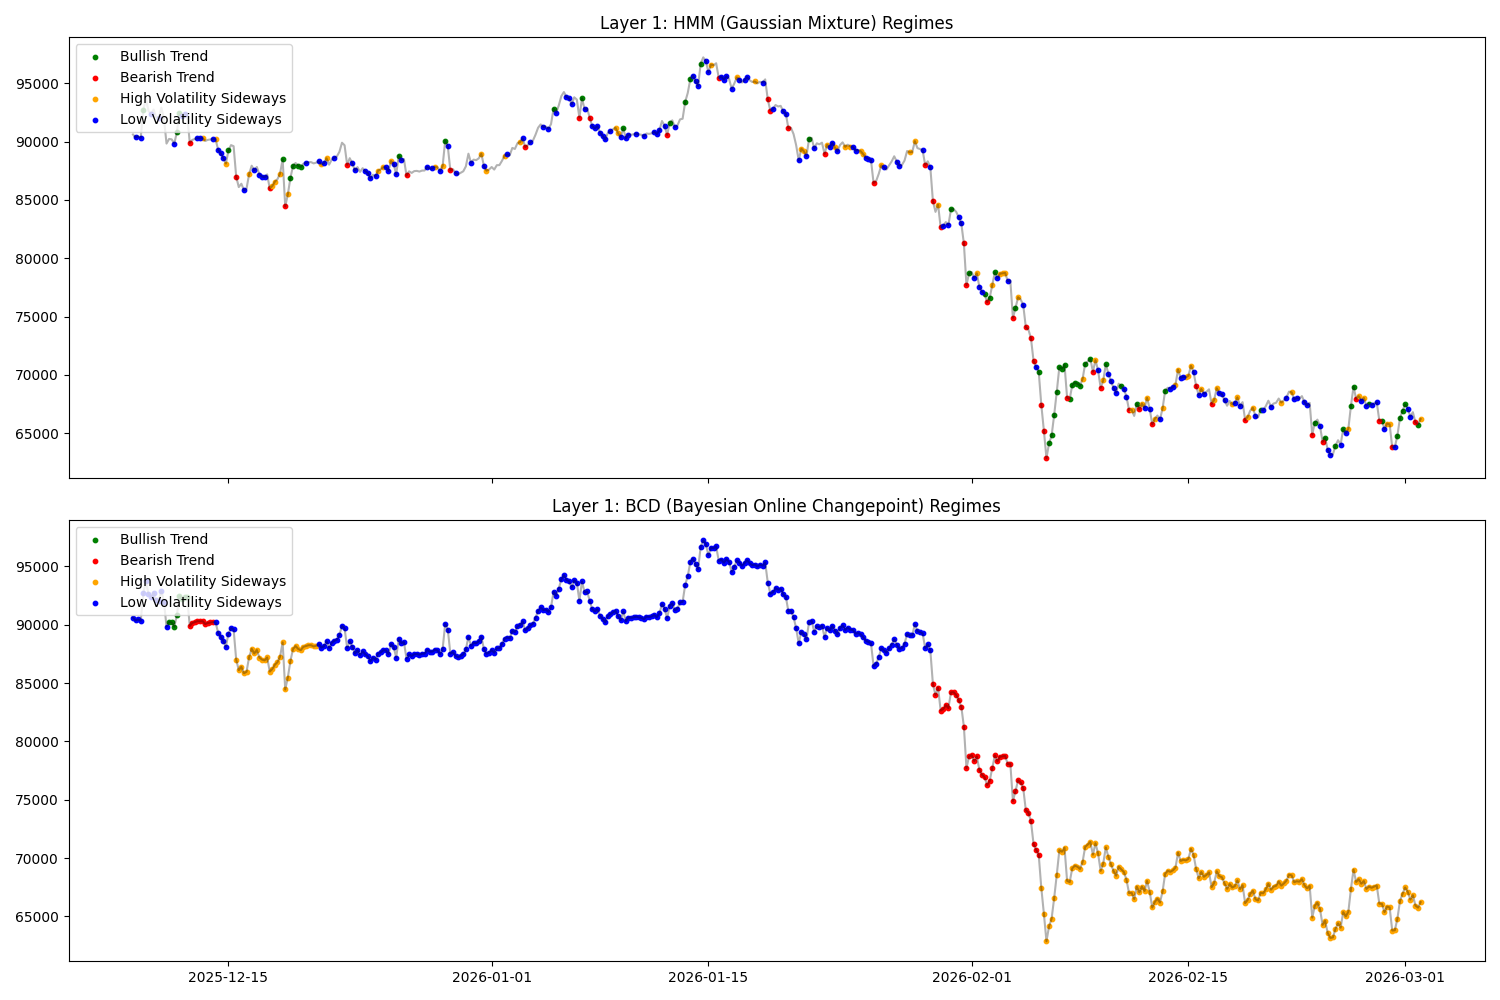
\includegraphics[width=0.8\textwidth]{figures/bcd_vs_hmm.png}
    \caption{Perbandingan Visual antara Deteksi Rezim HMM (Legacy) dan BCD (Ekonofisika).}
    \label{fig:hmm_vs_bcd}
\end{figure}

\subsection{Kegagalan Model Markovian}
Setelah melalui berbagai iterasi (\textit{Standard HMM}, \textit{Non-Homogeneous HMM}, dan \textit{GMM-HMM}), kami menemukan beberapa kelemahan fundamental:
\begin{enumerate}
    \item \textbf{Transition Rigidity:} Probabilitas transisi yang statis gagal menangkap perubahan mendadak akibat faktor eksternal seperti \textit{liquidation cascades} atau perubahan \textit{funding rate}.
    \item \textbf{High Latency/Bottleneck:} Model yang lebih kompleks (NHHM) membutuhkan waktu kalibrasi yang tidak realistis untuk sistem \textit{scalping} (berjam-jam per siklus).
    \item \textbf{Predictive Failure:} Melalui pengujian \textit{Walk-Forward} (Modul C), HMM secara konsisten gagal melewati ambang batas signifikansi statistik \textit{out-of-sample}.
\end{enumerate}

Kegagalan ini memicu pergeseran paradigma dari \textit{Machine Learning} murni ke arah pendekatan yang lebih fundamental: \textbf{Ekonofisika}.

\subsection{Struktur Dokumen}

Dokumen ini disusun sebagai berikut: Bab~\ref{sec:theory} menjelaskan landasan teoritis ekonofisika dan formulasi matematis BCD. Bab~\ref{sec:architecture} mendeskripsikan arsitektur 6-\textit{layer pipeline} secara menyeluruh. Bab~\ref{sec:evolution} mendokumentasikan evolusi sistem dari v0.1 hingga v4.5 beserta justifikasi empiris setiap transisi. Bab~\ref{sec:results} menyajikan validasi statistik komprehensif termasuk pengujian lintas regime dan perbandingan longitudinal. Bab~\ref{sec:conclusion} merangkum temuan dan memaparkan \textit{roadmap} pengembangan selanjutnya.
